\documentclass{beamer}
\usepackage{ctex, hyperref}
\usepackage[T1]{fontenc}
\usepackage{tikz}
\usetikzlibrary{arrows.meta, positioning}
% other packages
\usepackage{latexsym,amsmath,xcolor,multicol,booktabs,calligra}
\usepackage{graphicx,pstricks,listings,stackengine}

\usepackage{media9}

\author{谭诗弘，黄育民，曹洪珲}
\title{智能系统设计实践}
\subtitle{六足机器人避障控制\ 第二次进展汇报}
\institute{武汉大学电子信息学院}
\date{2025年10月13日}
\usepackage{whu}

% defs
\def\cmd#1{\texttt{\color{red}\footnotesize $\backslash$#1}}
\def\env#1{\texttt{\color{blue}\footnotesize #1}}
\definecolor{deepblue}{rgb}{0,0,0.5}
\definecolor{deepred}{rgb}{0.6,0,0}
\definecolor{deepgreen}{rgb}{0,0.5,0}
\definecolor{halfgray}{gray}{0.55}

\lstset{
    basicstyle=\ttfamily\small,
    keywordstyle=\bfseries\color{deepblue},
    emphstyle=\ttfamily\color{deepred},    % Custom highlighting style
    stringstyle=\color{deepgreen},
    numbers=left,
    numberstyle=\small\color{halfgray},
    rulesepcolor=\color{red!20!green!20!blue!20},
    frame=shadowbox,
}


\begin{document}

\kaishu
\begin{frame}
    \titlepage
    \begin{figure}[htpb]
        \begin{center}
            
\includegraphics[width=0.2\linewidth]{pic/whulogo.png}
        \end{center}
    \end{figure}
\end{frame}

\begin{frame}
    \tableofcontents[sectionstyle=show,subsectionstyle=show/shaded/hide,subsubsectionstyle=show/shaded/hide]
\end{frame}

\section{本周进展}

\begin{frame}{基于JupyterLab的基本运动代码实现和调试}
    \begin{itemize}
        \item 在六足机器人上部署成功了JupyterLab环境，实现了直接板上运行代码和调试。
        \item 参考资料成功实现了在Python环境中控制六足机器人的运动。
        \item 实现了六足机器人的前进、后退、左转、右转等基本运动。
        \item 调用实现了六足机器人的表演动作。
    \end{itemize}
\end{frame}

\begin{frame}{代码实现-库导入和机器人定义}

    Muto类负责整个机器人的协调，是机器人顶层类。
    \begin{figure}[htpb]
        \begin{center}
            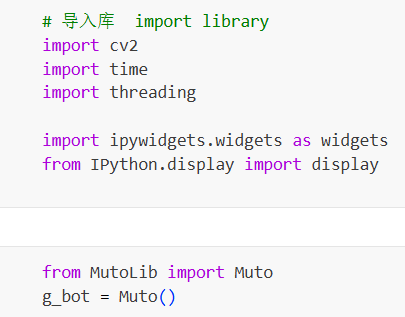
\includegraphics[width=0.49\linewidth]{pic/init.png}
        \end{center}
    \end{figure}
\end{frame}

\begin{frame}{代码实现-机器人控制}
    \begin{figure}[htpb]
        \begin{center}
            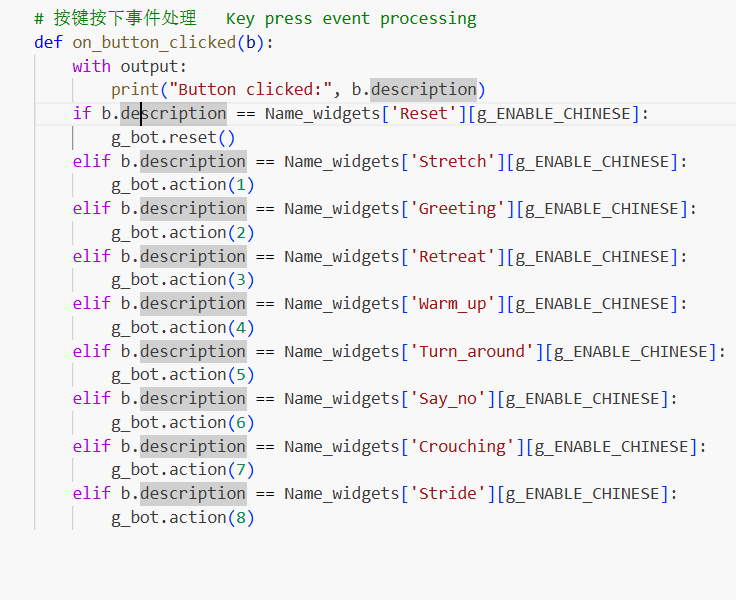
\includegraphics[width=0.49\linewidth]{pic/press1.png}
            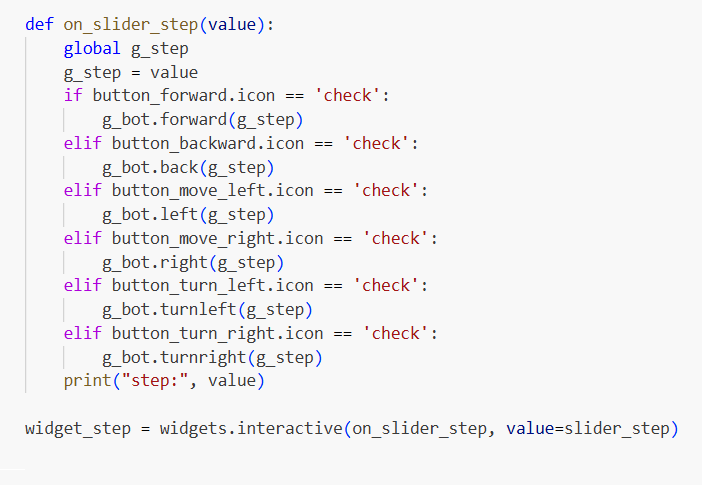
\includegraphics[width=0.49\linewidth]{pic/press2.png}
        \end{center}
    \end{figure}
\end{frame}

\begin{frame}{代码实现-机器人控制}
    \begin{figure}[htpb]
        \begin{center}
            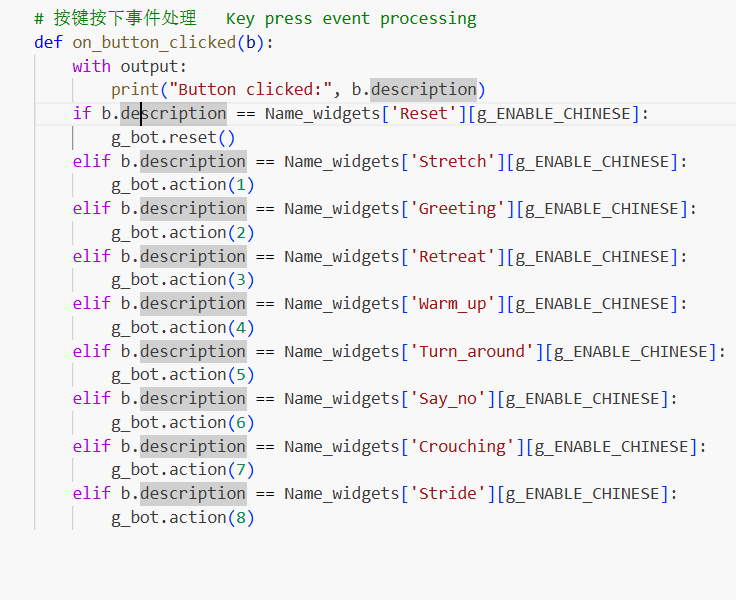
\includegraphics[width=0.49\linewidth]{pic/press1.png}
            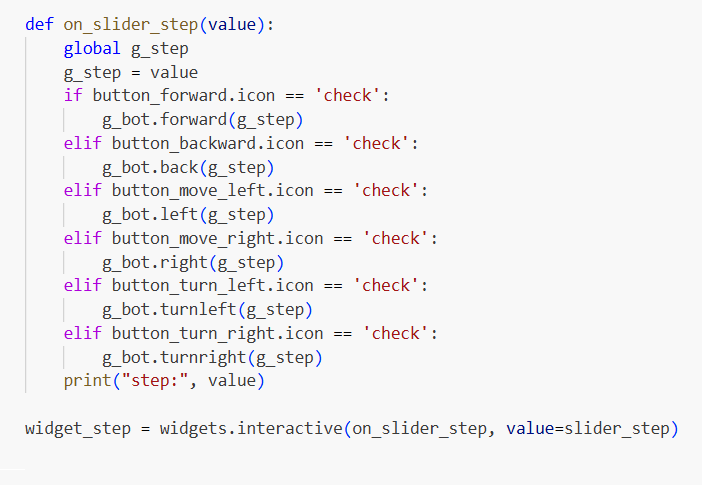
\includegraphics[width=0.49\linewidth]{pic/press2.png}
        \end{center}
    \end{figure}
\end{frame}

\begin{frame}{实现效果-表演动作}
    \begin{figure}[htpb]
        \begin{center}
            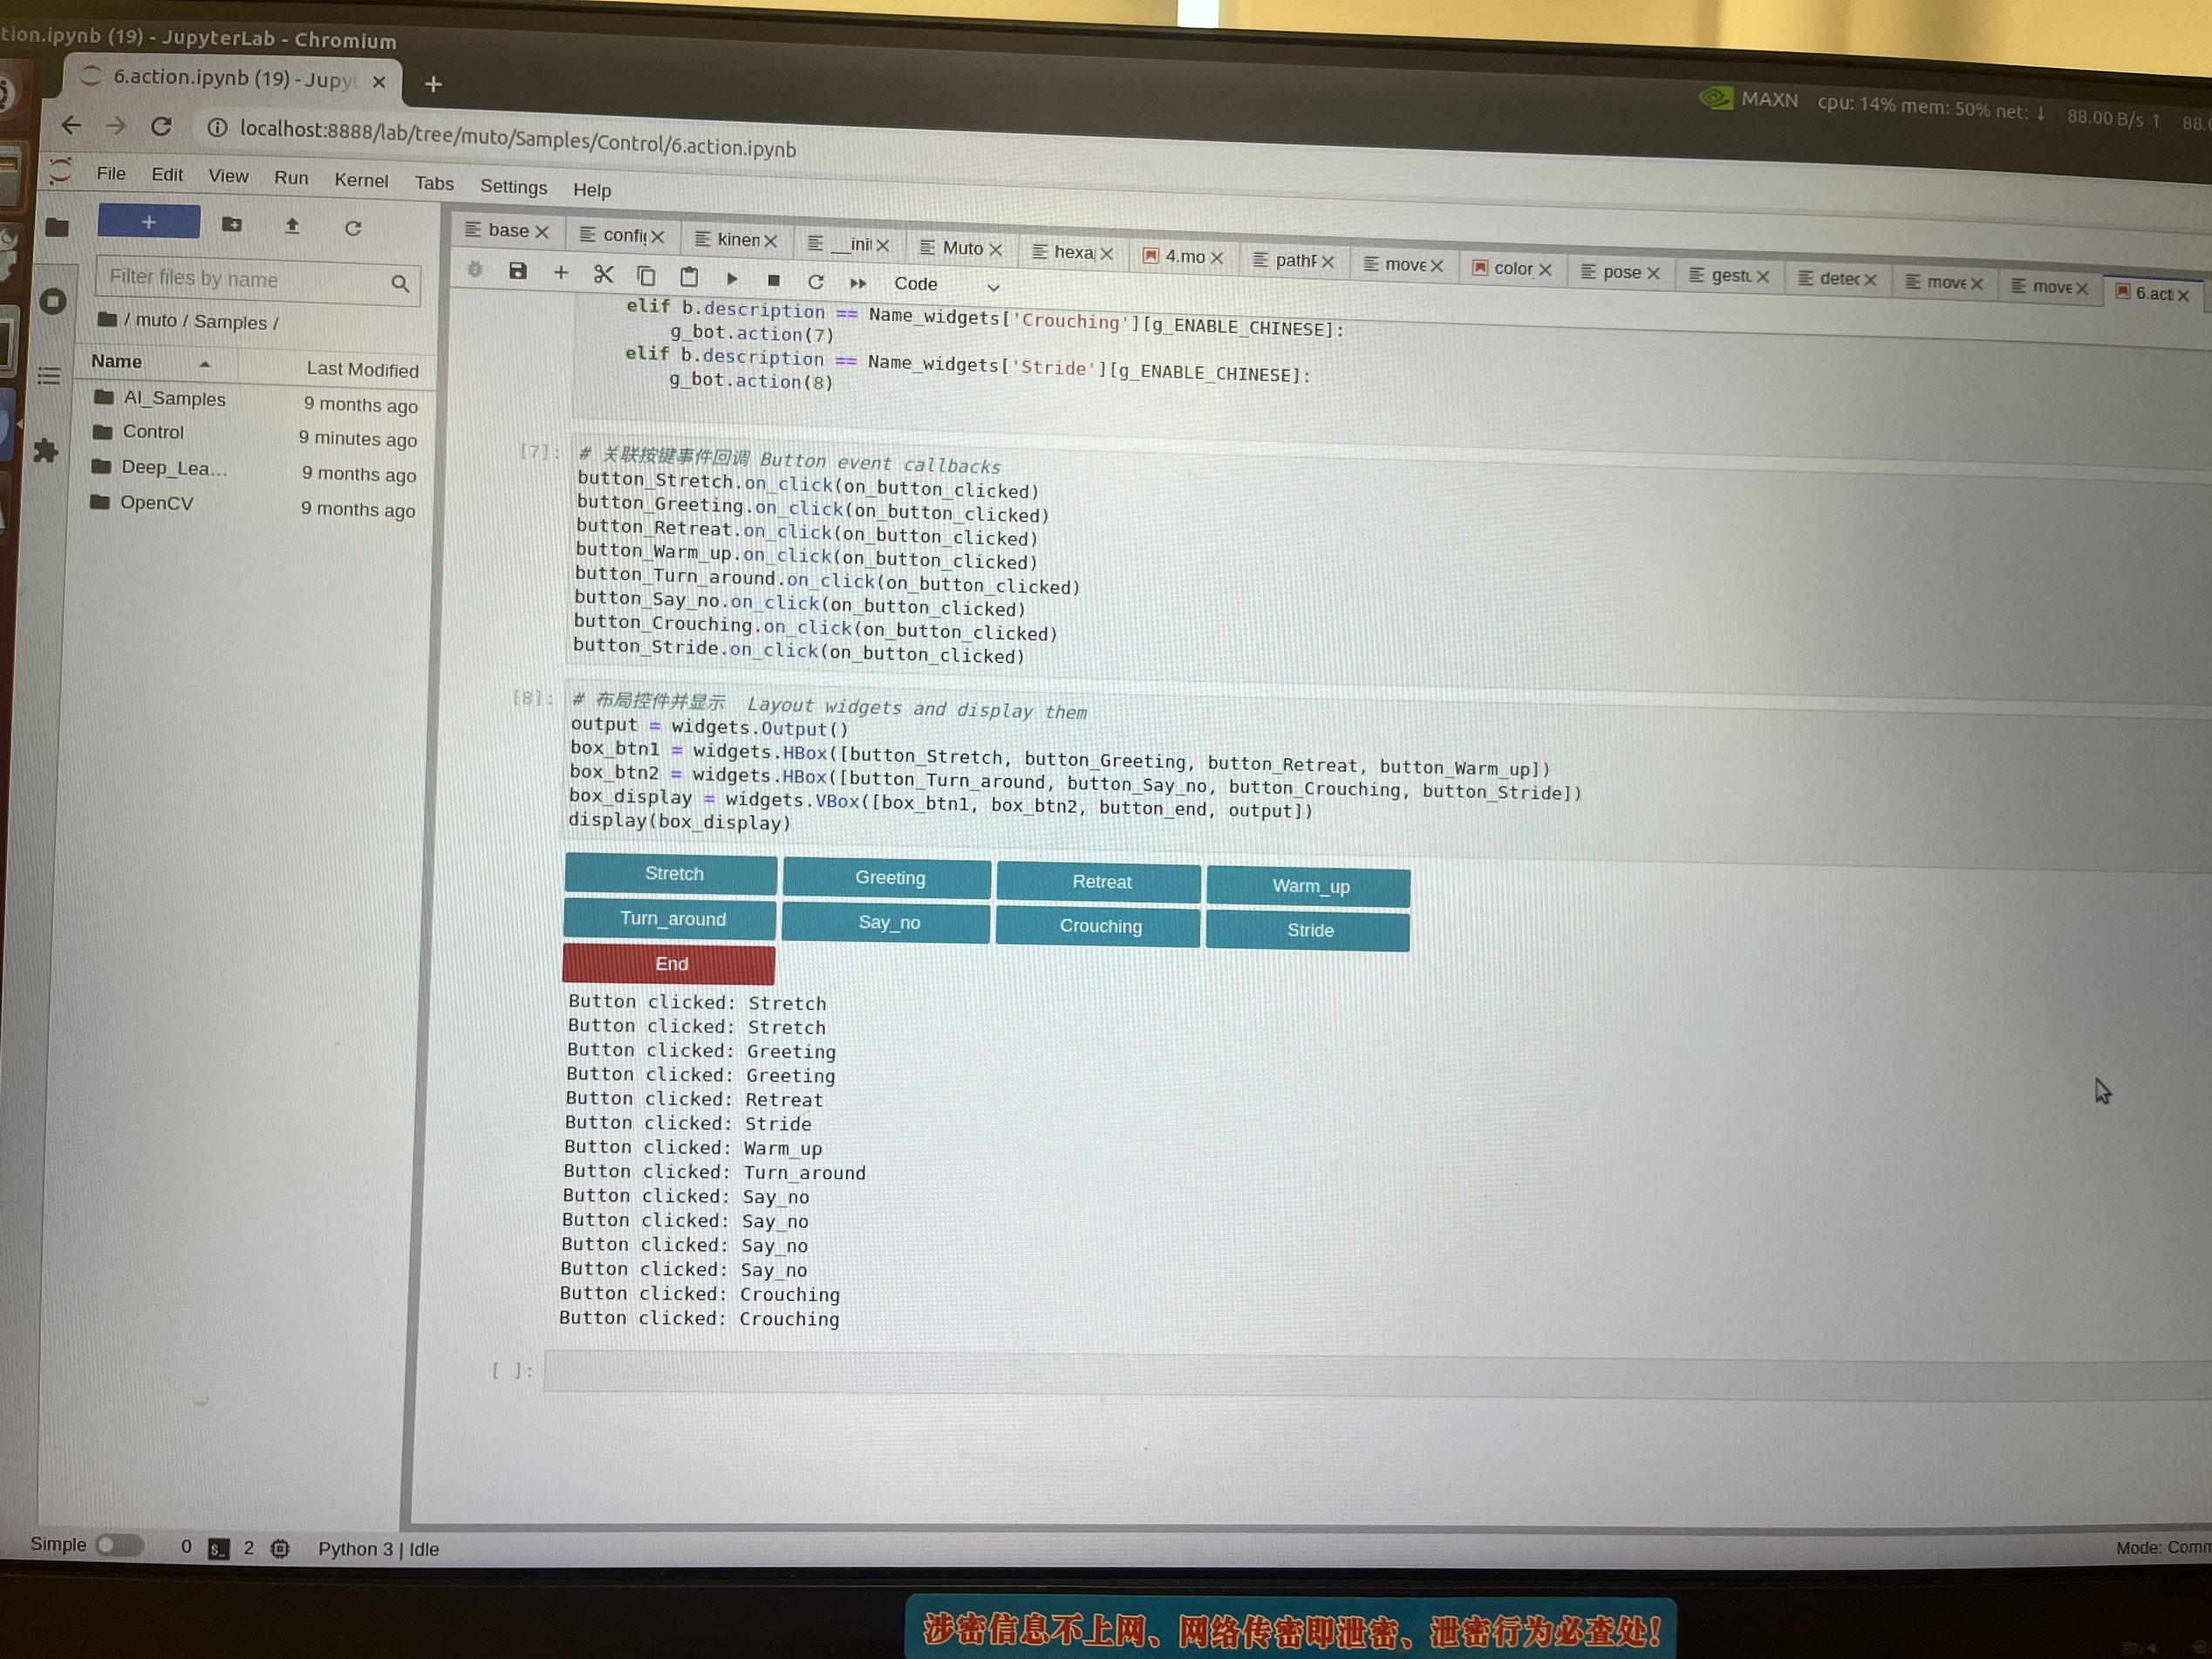
\includegraphics[width=0.8\linewidth]{pic/show1.jpg}
        \end{center}
    \end{figure}
\end{frame}

\begin{frame}{实现效果-基础控制}
    使用滑块空间来控制机器人的步长和速度。
    \begin{figure}[htpb]
        \begin{center}
            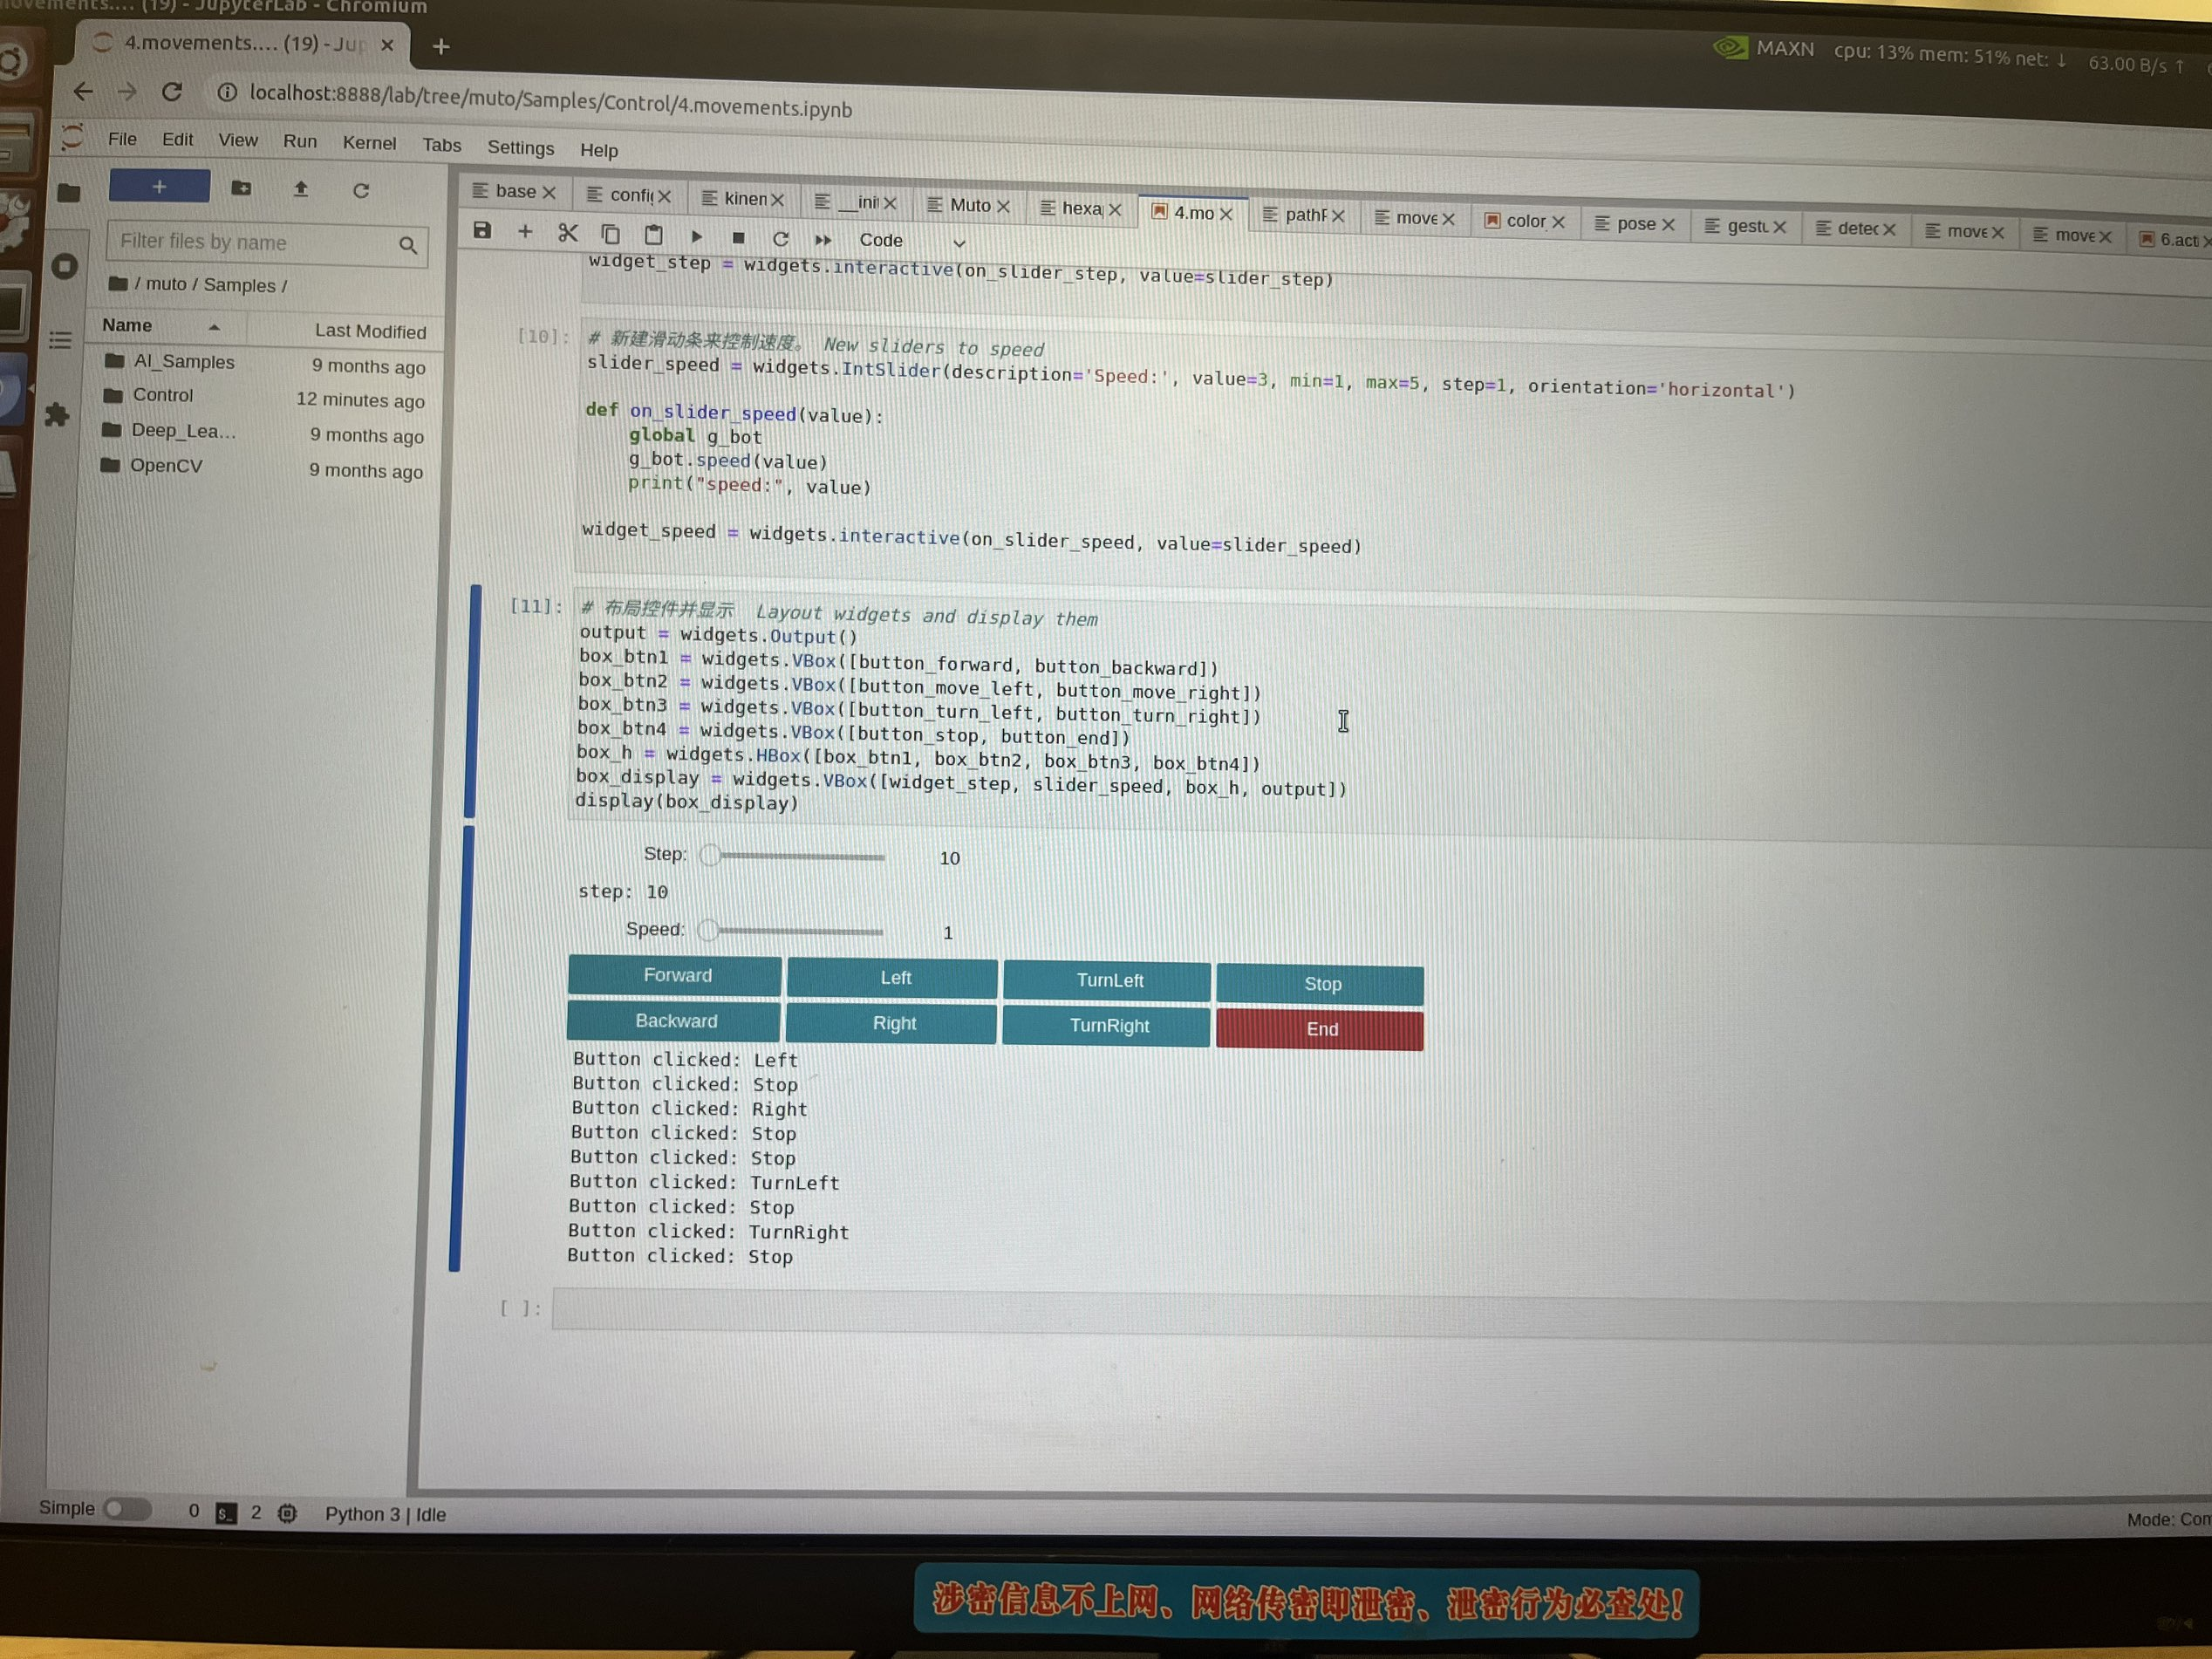
\includegraphics[width=0.8\linewidth]{pic/show2.jpg}
        \end{center}
    \end{figure}
\end{frame}

\begin{frame}{视频展示}
    \begin{center}
        {视频展示}
    \end{center}
\end{frame}

\section{后续规划}

\begin{frame}
    \begin{itemize}
        \item 对于底层代码进行修改，尝试改变机器人行走的步高等步态，实现自由控制。
        \item 调研相关文献资料，查询机器人足部控制相关代码。
        \item 实现机器人平稳上坡和下坡动作。
        \item 撰写中期报告。
    \end{itemize}
\end{frame}

\begin{frame}
    \begin{center}
        {\Huge\calligra Thanks!}
    \end{center}
\end{frame}

\end{document}